% Created by tikzDevice version 0.12.6 on 2025-04-16 10:40:40
% !TEX encoding = UTF-8 Unicode
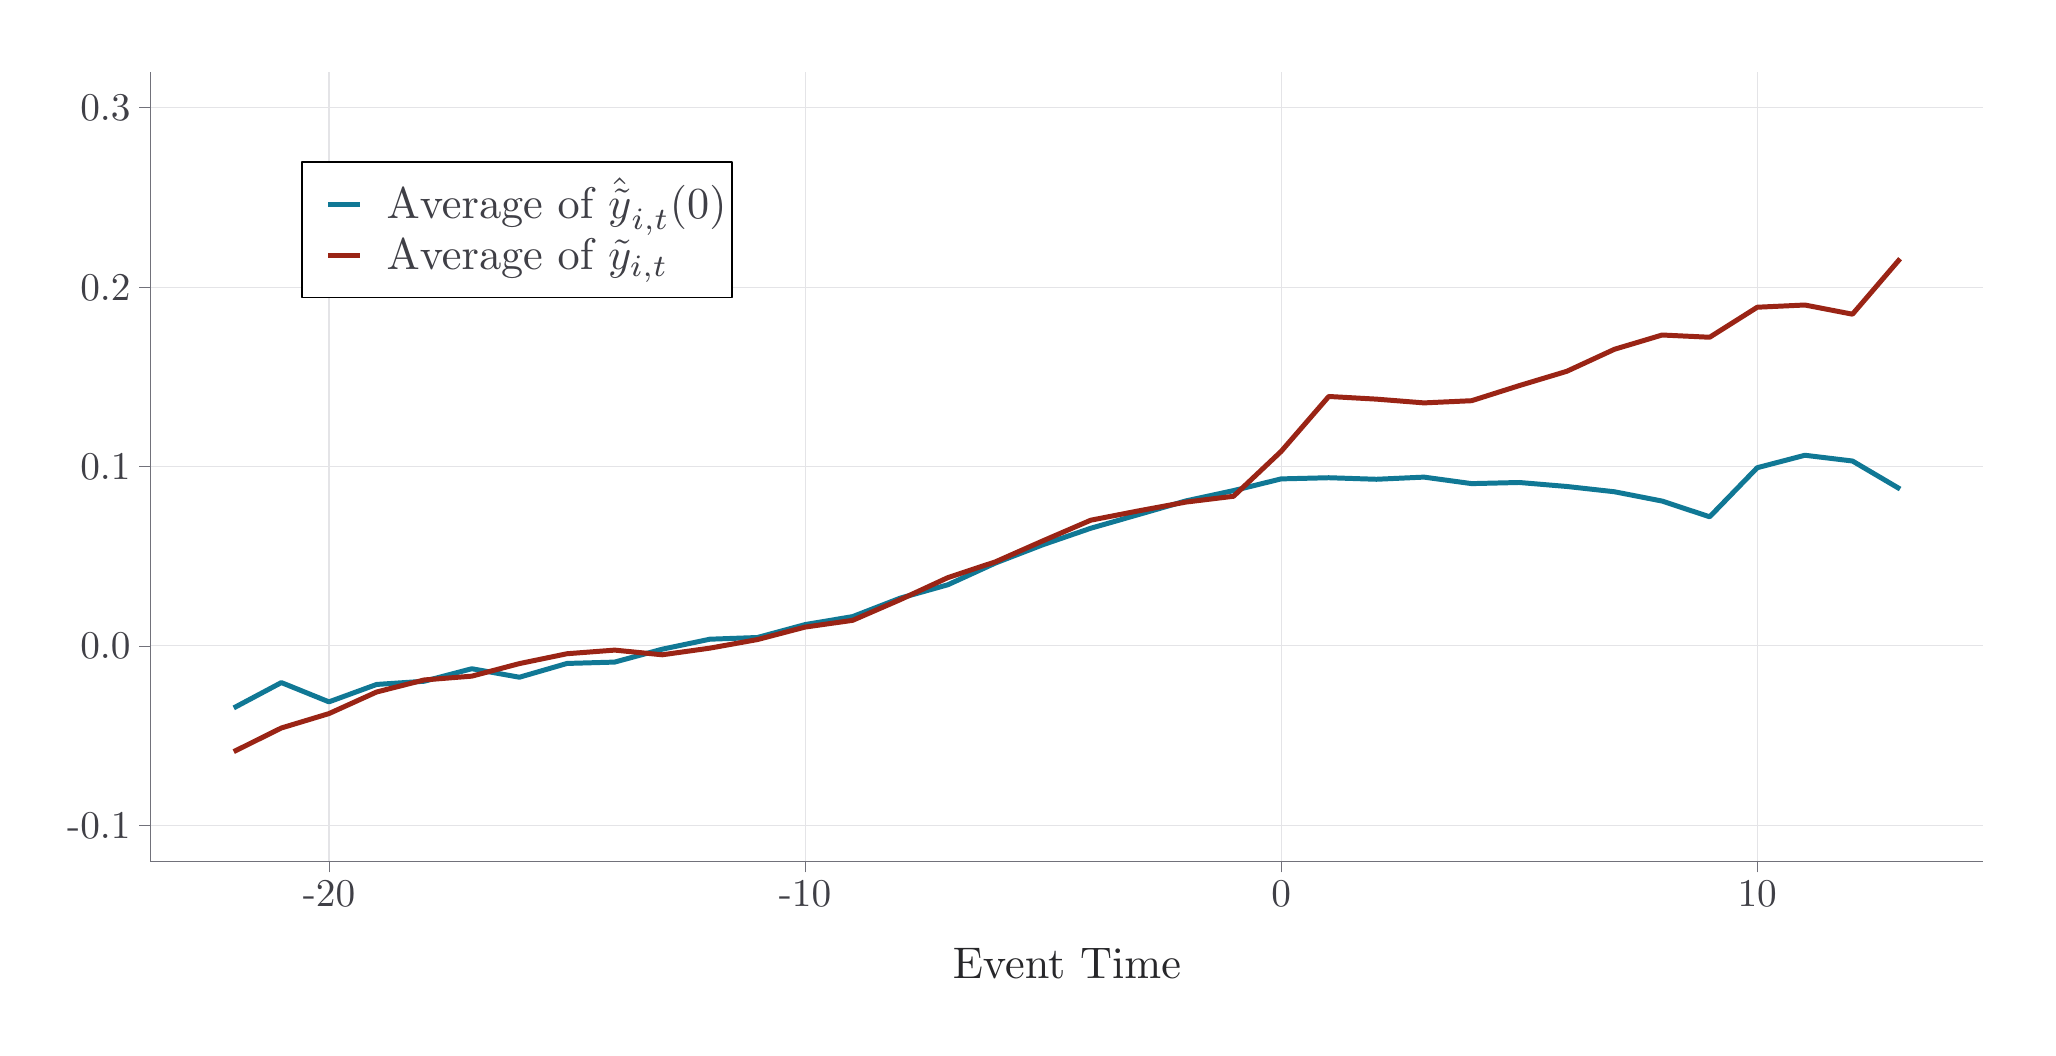
\begin{tikzpicture}[x=1pt,y=1pt]
\definecolor{fillColor}{RGB}{255,255,255}
\path[use as bounding box,fill=fillColor] (0,0) rectangle (722.70,361.35);
\begin{scope}
\path[clip] (  0.00,  0.00) rectangle (722.70,361.35);
\definecolor{drawColor}{RGB}{255,255,255}

\path[draw=drawColor,line width= 0.8pt,line join=round,line cap=round,fill=fillColor] (  0.00,  0.00) rectangle (722.70,361.35);
\end{scope}
\begin{scope}
\path[clip] ( 44.36, 60.16) rectangle (706.70,345.35);
\definecolor{drawColor}{RGB}{255,255,255}
\definecolor{fillColor}{RGB}{255,255,255}

\path[draw=drawColor,line width= 0.8pt,line join=round,line cap=round,fill=fillColor] ( 44.36, 60.16) rectangle (706.70,345.35);
\definecolor{drawColor}{RGB}{228,228,231}

\path[draw=drawColor,line width= 0.4pt,line join=round] ( 44.36, 73.12) --
	(706.70, 73.12);

\path[draw=drawColor,line width= 0.4pt,line join=round] ( 44.36,137.94) --
	(706.70,137.94);

\path[draw=drawColor,line width= 0.4pt,line join=round] ( 44.36,202.75) --
	(706.70,202.75);

\path[draw=drawColor,line width= 0.4pt,line join=round] ( 44.36,267.57) --
	(706.70,267.57);

\path[draw=drawColor,line width= 0.4pt,line join=round] ( 44.36,332.39) --
	(706.70,332.39);

\path[draw=drawColor,line width= 0.4pt,line join=round] (108.87, 60.16) --
	(108.87,345.35);

\path[draw=drawColor,line width= 0.4pt,line join=round] (280.91, 60.16) --
	(280.91,345.35);

\path[draw=drawColor,line width= 0.4pt,line join=round] (452.95, 60.16) --
	(452.95,345.35);

\path[draw=drawColor,line width= 0.4pt,line join=round] (624.98, 60.16) --
	(624.98,345.35);
\definecolor{drawColor}{RGB}{16,120,149}

\path[draw=drawColor,line width= 1.8pt,line join=round] ( 74.47,115.55) --
	( 91.67,124.70) --
	(108.87,117.73) --
	(126.08,124.02) --
	(143.28,125.18) --
	(160.48,129.70) --
	(177.69,126.63) --
	(194.89,131.61) --
	(212.09,132.10) --
	(229.30,136.76) --
	(246.50,140.37) --
	(263.71,140.99) --
	(280.91,145.65) --
	(298.11,148.54) --
	(315.32,155.22) --
	(332.52,160.05) --
	(349.72,167.91) --
	(366.93,174.54) --
	(384.13,180.46) --
	(401.34,185.39) --
	(418.54,190.35) --
	(435.74,194.07) --
	(452.95,198.30) --
	(470.15,198.72) --
	(487.35,198.16) --
	(504.56,198.94) --
	(521.76,196.59) --
	(538.96,197.00) --
	(556.17,195.56) --
	(573.37,193.65) --
	(590.58,190.29) --
	(607.78,184.60) --
	(624.98,202.34) --
	(642.19,206.84) --
	(659.39,204.76) --
	(676.59,194.63);
\definecolor{drawColor}{RGB}{154,36,21}

\path[draw=drawColor,line width= 1.8pt,line join=round] ( 74.47, 99.75) --
	( 91.67,108.29) --
	(108.87,113.49) --
	(126.08,121.29) --
	(143.28,125.65) --
	(160.48,127.02) --
	(177.69,131.56) --
	(194.89,135.12) --
	(212.09,136.43) --
	(229.30,134.74) --
	(246.50,137.14) --
	(263.71,140.24) --
	(280.91,144.75) --
	(298.11,147.19) --
	(315.32,154.67) --
	(332.52,162.63) --
	(349.72,168.34) --
	(366.93,175.95) --
	(384.13,183.37) --
	(401.34,186.73) --
	(418.54,189.92) --
	(435.74,192.02) --
	(452.95,208.25) --
	(470.15,228.08) --
	(487.35,227.12) --
	(504.56,225.76) --
	(521.76,226.55) --
	(538.96,232.00) --
	(556.17,237.18) --
	(573.37,245.13) --
	(590.58,250.29) --
	(607.78,249.48) --
	(624.98,260.33) --
	(642.19,261.13) --
	(659.39,257.81) --
	(676.59,277.85);
\end{scope}
\begin{scope}
\path[clip] (  0.00,  0.00) rectangle (722.70,361.35);
\definecolor{drawColor}{RGB}{113,113,122}

\path[draw=drawColor,line width= 0.3pt,line join=round] ( 44.36, 60.16) --
	( 44.36,345.35);
\end{scope}
\begin{scope}
\path[clip] (  0.00,  0.00) rectangle (722.70,361.35);
\definecolor{drawColor}{RGB}{63,63,70}

\node[text=drawColor,anchor=base east,inner sep=0pt, outer sep=0pt, scale=  1.42] at ( 37.16, 68.46) {-0.1};

\node[text=drawColor,anchor=base east,inner sep=0pt, outer sep=0pt, scale=  1.42] at ( 37.16,133.27) {0.0};

\node[text=drawColor,anchor=base east,inner sep=0pt, outer sep=0pt, scale=  1.42] at ( 37.16,198.09) {0.1};

\node[text=drawColor,anchor=base east,inner sep=0pt, outer sep=0pt, scale=  1.42] at ( 37.16,262.91) {0.2};

\node[text=drawColor,anchor=base east,inner sep=0pt, outer sep=0pt, scale=  1.42] at ( 37.16,327.72) {0.3};
\end{scope}
\begin{scope}
\path[clip] (  0.00,  0.00) rectangle (722.70,361.35);
\definecolor{drawColor}{RGB}{113,113,122}

\path[draw=drawColor,line width= 0.3pt,line join=round] ( 40.36, 73.12) --
	( 44.36, 73.12);

\path[draw=drawColor,line width= 0.3pt,line join=round] ( 40.36,137.94) --
	( 44.36,137.94);

\path[draw=drawColor,line width= 0.3pt,line join=round] ( 40.36,202.75) --
	( 44.36,202.75);

\path[draw=drawColor,line width= 0.3pt,line join=round] ( 40.36,267.57) --
	( 44.36,267.57);

\path[draw=drawColor,line width= 0.3pt,line join=round] ( 40.36,332.39) --
	( 44.36,332.39);
\end{scope}
\begin{scope}
\path[clip] (  0.00,  0.00) rectangle (722.70,361.35);
\definecolor{drawColor}{RGB}{113,113,122}

\path[draw=drawColor,line width= 0.3pt,line join=round] ( 44.36, 60.16) --
	(706.70, 60.16);
\end{scope}
\begin{scope}
\path[clip] (  0.00,  0.00) rectangle (722.70,361.35);
\definecolor{drawColor}{RGB}{113,113,122}

\path[draw=drawColor,line width= 0.3pt,line join=round] (108.87, 56.16) --
	(108.87, 60.16);

\path[draw=drawColor,line width= 0.3pt,line join=round] (280.91, 56.16) --
	(280.91, 60.16);

\path[draw=drawColor,line width= 0.3pt,line join=round] (452.95, 56.16) --
	(452.95, 60.16);

\path[draw=drawColor,line width= 0.3pt,line join=round] (624.98, 56.16) --
	(624.98, 60.16);
\end{scope}
\begin{scope}
\path[clip] (  0.00,  0.00) rectangle (722.70,361.35);
\definecolor{drawColor}{RGB}{63,63,70}

\node[text=drawColor,anchor=base,inner sep=0pt, outer sep=0pt, scale=  1.42] at (108.87, 43.63) {-20};

\node[text=drawColor,anchor=base,inner sep=0pt, outer sep=0pt, scale=  1.42] at (280.91, 43.63) {-10};

\node[text=drawColor,anchor=base,inner sep=0pt, outer sep=0pt, scale=  1.42] at (452.95, 43.63) {0};

\node[text=drawColor,anchor=base,inner sep=0pt, outer sep=0pt, scale=  1.42] at (624.98, 43.63) {10};
\end{scope}
\begin{scope}
\path[clip] (  0.00,  0.00) rectangle (722.70,361.35);
\definecolor{drawColor}{RGB}{39,39,42}

\node[text=drawColor,anchor=base,inner sep=0pt, outer sep=0pt, scale=  1.60] at (375.53, 17.89) {Event Time};
\end{scope}
\begin{scope}
\path[clip] (  0.00,  0.00) rectangle (722.70,361.35);
\definecolor{drawColor}{RGB}{0,0,0}
\definecolor{fillColor}{RGB}{255,255,255}

\path[draw=drawColor,line width= 0.6pt,line join=round,line cap=round,fill=fillColor] ( 99.23,263.86) rectangle (254.43,312.77);
\end{scope}
\begin{scope}
\path[clip] (  0.00,  0.00) rectangle (722.70,361.35);
\definecolor{drawColor}{RGB}{255,255,255}
\definecolor{fillColor}{RGB}{255,255,255}

\path[draw=drawColor,line width= 0.8pt,line join=round,line cap=round,fill=fillColor] (107.23,290.31) rectangle (121.68,304.77);
\definecolor{drawColor}{RGB}{16,120,149}

\path[draw=drawColor,line width= 1.8pt,line join=round] (108.67,297.54) -- (120.24,297.54);
\end{scope}
\begin{scope}
\path[clip] (  0.00,  0.00) rectangle (722.70,361.35);
\definecolor{drawColor}{RGB}{255,255,255}
\definecolor{fillColor}{RGB}{255,255,255}

\path[draw=drawColor,line width= 0.8pt,line join=round,line cap=round,fill=fillColor] (107.23,271.86) rectangle (121.68,286.31);
\definecolor{drawColor}{RGB}{154,36,21}

\path[draw=drawColor,line width= 1.8pt,line join=round] (108.67,279.08) -- (120.24,279.08);
\end{scope}
\begin{scope}
\path[clip] (  0.00,  0.00) rectangle (722.70,361.35);
\definecolor{drawColor}{RGB}{63,63,70}

\node[text=drawColor,anchor=base west,inner sep=0pt, outer sep=0pt, scale=  1.60] at (129.68,292.29) {Average of $\hat{\tilde{y}}_{i,t}(0)$};
\end{scope}
\begin{scope}
\path[clip] (  0.00,  0.00) rectangle (722.70,361.35);
\definecolor{drawColor}{RGB}{63,63,70}

\node[text=drawColor,anchor=base west,inner sep=0pt, outer sep=0pt, scale=  1.60] at (129.68,273.84) {Average of $\tilde{y}_{i,t}$};
\end{scope}
\end{tikzpicture}
